\documentclass{article}
\usepackage{fancyhdr}
\usepackage{titlesec}
\usepackage{graphicx}
\usepackage[dvipsnames]{xcolor}
\graphicspath{ {./img/} }

\pagestyle{fancy}
\fancyhf{}
\lhead{Modul 1 Praktikum Jaringan Komputer}
\rfoot{\footnotesize Page \thepage}
\lfoot{\footnotesize Mahyus Ihsan, S.Si, M.Si \newline Jurusan Informatika Universitas Syiah Kuala \newline Modul oleh : Diky Wahyudi, Furqan Al Ghifari, Rendika Rahmaturrizki}
\renewcommand{\headrulewidth}{1pt}
\renewcommand{\footrulewidth}{1pt}

\titleformat*{\section}{\small\bfseries}

\begin{document}
    \begin{center}
        \textbf{Modul 5 Praktikum Jaringan Komputer}

        \textbf{IPv6}
    \end{center}

    \section*{Deskripsi Singkat}
    IPv6 adalah versi terbaru dari Protokol Internet, protokol komunikasi yang menyediakan sistem identifikasi dan lokasi untuk komputer di jaringan dan merutekan lalu lintas di Internet. IPv6 dikembangkan oleh Internet Engineering Task Force untuk menangani masalah kelelahan alamat IPv4 yang telah lama diantisipasi. 
    \section*{Tujuan}
    \begin{enumerate}
        \item Dapat memahami struktur dan jenis- jenis dari IPv6
        \item Dapat memahani tentang \textit{subnetting} dan implementasikan pengalamatan pada IPv6
        \item Dapat memahami dan melakukan \textit{Unicast dan Broadcast} pada IPv6
    \end{enumerate}

    \begin{flushleft}
        \textbf{Materi 1 - Struktur IPv6}
        \newline

        IPv6 memiliki panjang \textbf{128bits} dan ditulis dalam 8 bagian dan setiap bagian mengandung 16bits yang ditulis dalam 4bit bilangan \textbf{hexadecimal}.

        \begin{center}
            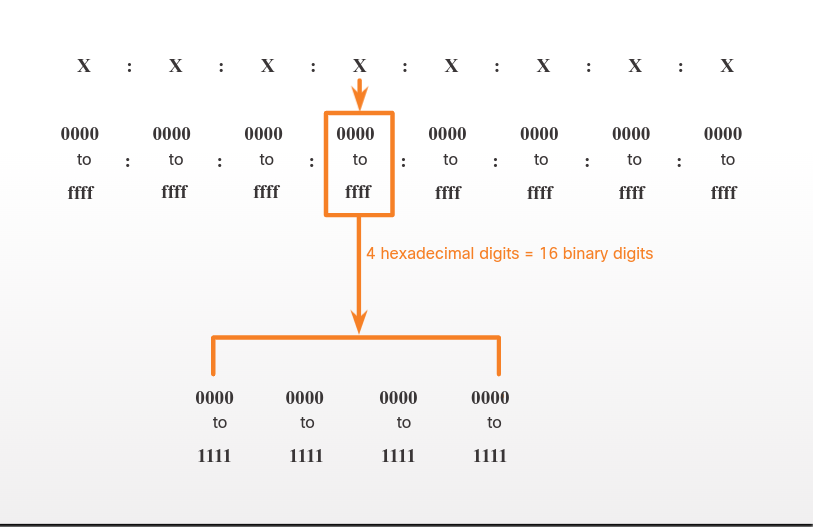
\includegraphics[scale=0.5]{1-1.png}
        \end{center}
        
        Contoh IPv6 
        \begin{center}
            \textbf{2001 : 0db8 : 0000 : 00a3 : ab00 : 0ab0 : 00ab : 1234}
            \newline
        \end{center}

        \textbf{Aturan dalam menulis IPv6}
        \begin{itemize}
            \item[] \textbf{Prefered Format} \newline
            Prefered format adalah cara penulisan IPv6 secara menyeluruh yaitu dengan menggunakan \textbf{32bit bilangan hexadecimal}
            \begin{center}
                2001 : 0db8 : 0000 : 00a3 : ab00 : 0ab0 : 00ab : 1234
            \end{center}
            Semua bit pada IPv6 dituliskan dengan 8 bagian yang antar bagian dibatasi dengan tanda titik koma (;)

            \item[] \textbf{Omit Leading Zeros} \newline
            Omit Leading Zeros adalah pengurangan bilangan 0 yang berada di depan untuk menyingkat penulisan IPv6
            \begin{center}
                2001 : 0db8 : 0000 : 00a3 : ab00 : 0ab0 : 00ab : 1234
            \end{center}
            
            Setelah Omit Leading Zero
            \begin{center}
                2001 : db8 : 0 : a3 : ab00 : ab0 : ab : 1234
            \end{center}

            \item[] \textbf{Double Colon} \newline
            Double Colon adalah penggunaan dua buah tanda titik dua (::) untuk mempersingkat sebuah grup angka 0
            \begin{center}
                2001 : 0db8 : 0000 : 1111 : \textcolor{red}{0000 : 0000 : 0000} : 0200
            \end{center}

            Setelah di sederhanakan menggunakan Omit Leading Zero dan Double Colon akan menjadi
            \begin{center}
                2001 : db8 : 0 : 1111 :: 0200
            \end{center}

            Jika terdapat lebih dari 1 grup angka 0 maka Double Colon akan digunakan pada grup yang paling panjang dan jika mereka sama grup yang pertama kali akan meggunakan Double Colon
            \begin{center}
                2001 : 0db8 : \textcolor{red}{0000 : 0000} : ab00 : \textcolor{red}{0000 : 0000} : 0012
            \end{center}

            Maka akan menjadi
            \begin{center}
                2001 : db8 :: ab00 : 0 : 0 : 12 
            \end{center}
        \end{itemize}
        \newpage
        
        Contoh melakukan \textbf{compress} pada sebuah IPv6
        \begin{itemize}
            \item[] Prefered
            \begin{center}
                2001 : 0db8 : \textcolor{red}{0000 : 0000} : ab00 : \textcolor{red}{0000 : 0000 : 0000}
            \end{center}
            \item[] Omit Leading Zero
            \begin{center}
                2001 : db8 : 0 : 0 : ab00 : 0 : 0 : 0
            \end{center}
            \item[] Double Colon
            \begin{center}
                2001 : db8 : 0 : 0 : ab00 ::
            \end{center}
        \end{itemize}
    \end{flushleft}

    \begin{flushleft}
        \textbf{Materi 2 - NamaMateri}
        \newline

        Isi materi 2
    \end{flushleft}

    \begin{flushleft}
        \textbf{Materi 3 - NamaMateri}
        \newline

        Isi materi 3
    \end{flushleft}

    \newpage
    \begin{flushleft}
        \textbf{Tugas}
        \newline

        \begin{enumerate}
            \item Tugas 1
            \item Tugas 2
        \end{enumerate}
    \end{flushleft}
\end{document}
